\documentclass[11pt]{article}
\usepackage[margin=1in]{geometry}
\usepackage{amsmath,amssymb,bm}
\usepackage{tikz}
\usetikzlibrary{arrows.meta}
\usepackage{hyperref}
\usepackage{enumitem}
\usepackage{booktabs}
\usepackage{float}

\newcommand{\vect}[1]{\bm{#1}}
\newcommand{\uv}[1]{\hat{\bm{#1}}}
\newcommand{\xhat}{\uv{x}}
\newcommand{\yhat}{\uv{y}}
\newcommand{\zhat}{\uv{z}}
\newcommand{\nf}{\uv{n}_{\!f}}
\newcommand{\nr}{\uv{n}_{\!r}}
\newcommand{\bfh}{\uv{b}_{\!f}}
\newcommand{\brh}{\uv{b}_{\!r}}
\newcommand{\efh}{\uv{e}_{\!f}}
\newcommand{\erh}{\uv{e}_{\!r}}

\title{The Cat Righting Reflex:\\
Full-Cylinder and Half-Cylinder Models\\with No-Wringing Constraint}
\author{D.\ Carlsmith, with computational assistance from Claude (Anthropic)}
\date{March 2026}

\begin{document}
\maketitle

\begin{abstract}
We analyze the cat righting reflex using two models: (I)~two identical
full cylinders joined at a fixed bend angle~$\theta$, and (II)~two
identical half-cylinders (the belly halves) with a center-of-mass offset
from the geometric axis.  Working entirely in Cartesian coordinates with
the origin at the system center of mass, we compute the total angular
momentum by explicit integration over mass elements.  The no-wringing
constraint---equal and opposite spin rates about outward-pointing
axes---determines a unique whole-body counter-rotation (the righting
flip) that maintains zero total angular momentum.  We derive the gearing
ratio for each model, specialize to $\theta=90^\circ$, and show that the
half-cylinder gearing is suppressed by the factor
$1-32/(9\pi^2)\approx0.640$, equal to the ratio of axial moments of
inertia.  We then derive the internal torques at the joint in both
cases, decomposing each into spin, orbital, and whole-body-rotation
contributions. Every formula is verified by independent SymPy symbolic
integration.  Detailed calculations are provided in the appendices so
that the reader may check every step.
\end{abstract}

\tableofcontents

%======================================================================
\section{Introduction}
%======================================================================

A cat released upside-down in free fall can right itself and land on its
feet, even with zero initial angular momentum.  The simplest mechanical
model replaces the cat with two rigid cylinders joined at a fixed bend
angle, each spinning about its own axis in opposite senses (the
``no-wringing'' constraint).  Because the two spin axes are non-parallel,
the spin angular momenta do not cancel vectorially, and a compensating
whole-body rotation about the arch axis is required to maintain
$\vect{L}=\vect{0}$.  This compensating rotation is the righting flip.

We treat two variants of this model: full cylinders
(Section~\ref{sec:full}) and half-cylinders (Section~\ref{sec:half}).
The half-cylinder model represents a cat whose cross-section is
semicircular (the belly side only), introducing a center-of-mass offset
$\delta=4R/(3\pi)$ from the geometric axis.  We compare the gearing
ratios (Section~\ref{sec:compare}), derive the internal torques
(Section~\ref{sec:torques}), and present complete step-by-step
calculations in the appendices.

%======================================================================
\section{Common Setup}
\label{sec:setup}
%======================================================================

\subsection{Coordinate system}

The origin is at the system center of mass.  The $y$-axis points along
the symmetry axis of the arch (upward, from the system center of mass
toward the joint), $x$ is horizontal (the flip axis), and $z$ completes
the right-handed system.  The half-angle is $\alpha\equiv\theta/2$.
The outward-pointing axis unit vectors are
\begin{equation}\label{eq:axes}
\nf = (\sin\alpha,\;\cos\alpha,\;0), \qquad
\nr = (-\sin\alpha,\;\cos\alpha,\;0).
\end{equation}

\subsection{The no-wringing constraint}

The front cylinder spins at $+\omega$ about~$\nf$ and the rear at
$-\omega$ about~$\nr$.  This ensures material continuity at the
joint---no relative twist.

\subsection{Perpendicular basis vectors}

For each cylinder we need two directions perpendicular to the axis:
\begin{align}
\uv{e}_1 &= \zhat = (0,0,1), \label{eq:e1}\\
\uv{e}_{2f} &= \nf\times\zhat = (\cos\alpha,-\sin\alpha,0), \label{eq:e2f}\\
\uv{e}_{2r} &= \nr\times\zhat = (\cos\alpha,\sin\alpha,0). \label{eq:e2r}
\end{align}
The cross-product relations are:
\begin{equation}\label{eq:crossrels}
\nf\times\uv{e}_1 = \uv{e}_{2f},\qquad
\nf\times\uv{e}_{2f} = -\uv{e}_1.
\end{equation}

%======================================================================
\section{Model~I: Full Cylinders}
\label{sec:full}
%======================================================================

\subsection{Geometry}

Two identical uniform cylinders of mass~$m$, length~$\ell=s_2-s_1$,
and radius~$R$ are joined at a bend with fixed opening angle~$\theta$.
Each cylinder is parameterized by arc-length~$s$ from $s_1$ to~$s_2$
measured from the joint; the gap $s_1=R/\tan\alpha$ prevents overlap.
(See Figure~\ref{fig:full_geom}.)

\begin{figure}[H]
\centering
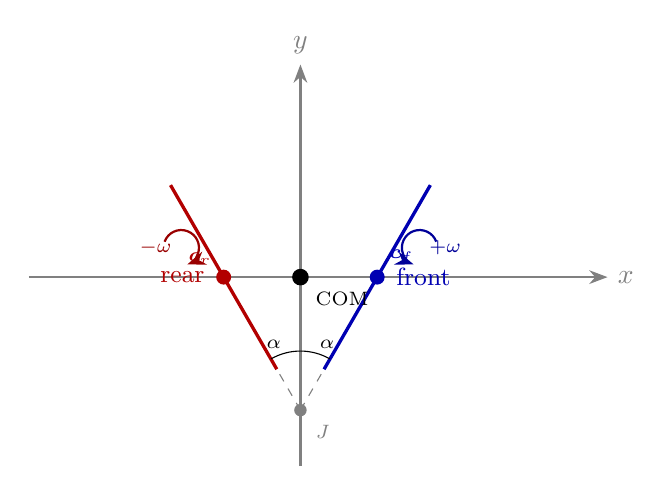
\begin{tikzpicture}[scale=1.5, >=Stealth]
  \draw[->, thick, gray] (-2.3,0) -- (2.6,0) node[right]{$x$};
  \draw[->, thick, gray] (0,-1.6) -- (0,1.8) node[above]{$y$};
  \coordinate (J) at (0,-1.126);
  \draw[very thick, blue!70!black] (0.2,-0.78) -- (1.1,0.779)
    node[pos=0.5, right=3pt]{\small front};
  \draw[very thick, red!70!black] (-0.2,-0.78) -- (-1.1,0.779)
    node[pos=0.5, left=3pt]{\small rear};
  \draw[thin, gray, dashed] (J) -- (0.2,-0.78);
  \draw[thin, gray, dashed] (J) -- (-0.2,-0.78);
  \fill[blue!70!black] (0.65, 0) circle (1.8pt)
    node[above right=1pt]{\scriptsize $\vect{c}_f$};
  \fill[red!70!black] (-0.65, 0) circle (1.8pt)
    node[above left=1pt]{\scriptsize $\vect{c}_r$};
  \fill[black] (0,0) circle (2pt) node[below right=2pt]{\scriptsize COM};
  \fill[black!50] (J) circle (1.5pt) node[below right=2pt]{\scriptsize $J$};
  \draw[thin] (0,-1.126+0.5) arc (90:60:0.5)
    node[pos=0.5, above right=-2pt]{\scriptsize $\alpha$};
  \draw[thin] (0,-1.126+0.5) arc (90:120:0.5)
    node[pos=0.5, above left=-2pt]{\scriptsize $\alpha$};
  \draw[->, thick, blue!60!black] (1.15, 0.3) arc (20:250:0.15)
    node[right, xshift=2pt, yshift=6pt]{\scriptsize $+\omega$};
  \draw[->, thick, red!60!black] (-1.15, 0.3) arc (160:-70:0.15)
    node[left, xshift=-2pt, yshift=6pt]{\scriptsize $-\omega$};
\end{tikzpicture}
\caption{Full-cylinder model.  Both cylinder centers of mass lie on the $x$-axis.}
\label{fig:full_geom}
\end{figure}

The center of mass of each cylinder is at distance
$\bar{s}=(s_1+s_2)/2$ along its axis from the joint.  Setting the
origin at the system center of mass:
\begin{equation}\label{eq:full_com}
J = (0,-\bar{s}\cos\alpha,0),\quad
\vect{c}_f = (+\bar{s}\sin\alpha,0,0),\quad
\vect{c}_r = (-\bar{s}\sin\alpha,0,0).
\end{equation}
Both cylinder centers lie on the $x$-axis.

\subsection{Angular momentum}

A mass element at position
$\vect{p}=J+s\,\nf+\rho\,\uv{e}_\perp(\phi)$ in the front cylinder
(with $\uv{e}_\perp=\cos\phi\,\uv{e}_{2f}+\sin\phi\,\uv{e}_1$,
$\phi\in[0,2\pi)$) has velocity
$\vect{v}=\vect{v}_{\rm spin}+\vect{\Omega}\times\vect{p}$.  The
spin velocity is
$\vect{v}_{\rm spin}=\omega\rho(\sin\phi\,\uv{e}_{2f}-\cos\phi\,\uv{e}_1)$.

The complete integration (Appendix~\ref{app:full}) yields, with the
no-wringing constraint:
\begin{align}
L_x &= \frac{m}{6}\bigl[
  \Omega_x\,\mathcal{I}_{xx}^{(\rm full)}
  + 6R^2\omega\sin\alpha\bigr], \label{eq:Lx_full}\\
L_y &= \frac{m}{6}\,\Omega_y\,\mathcal{I}_{yy}^{(\rm full)},
  \label{eq:Ly_full}\\
L_z &= \frac{m}{6}\,\Omega_z\,\mathcal{I}_{zz}^{(\rm full)},
  \label{eq:Lz_full}
\end{align}
where
\begin{align}
\mathcal{I}_{xx}^{(\rm full)} &= (\ell^2-3R^2)\cos^2\!\alpha+6R^2, \label{eq:Ixx_full}\\
\mathcal{I}_{yy}^{(\rm full)} &= (\ell^2+12\bar{s}^2-3R^2)\sin^2\!\alpha+6R^2, \label{eq:Iyy_full}\\
\mathcal{I}_{zz}^{(\rm full)} &= \ell^2+12\bar{s}^2\sin^2\!\alpha+3R^2. \label{eq:Izz_full}
\end{align}
The spin term appears \emph{only} in $L_x$, and
$\mathcal{I}_{xx}^{(\rm full)}$ has no $\bar{s}$-dependence (the
cylinder centers lie on the $x$-axis).

\subsection{Gearing ratio}

Setting $\vect{L}=\vect{0}$: $\Omega_y=\Omega_z=0$ and
\begin{equation}\label{eq:gear_full}
\boxed{\;
\frac{\Omega_x}{\omega}\bigg|_{\rm full}
= -\frac{6R^2\sin\alpha}
  {(\ell^2-3R^2)\cos^2\!\alpha+6R^2}\;.}
\end{equation}

%======================================================================
\section{Model~II: Half-Cylinders}
\label{sec:half}
%======================================================================

\subsection{Geometry}

Each half-cylinder is the top half ($\phi\in[0,\pi]$) of radius~$R$,
length~$L$, mass~$m$.  Each extends outward from the joint ($s\in[0,L]$).
In addition to the perpendicular basis $(\uv{e}_1,\uv{e}_{2f})$, we
define the ``belly'' direction (from the geometric axis toward the
half-disk center of mass):
\begin{equation}
\bfh = (\cos\alpha,-\sin\alpha,0),\qquad
\brh = (-\cos\alpha,-\sin\alpha,0).
\end{equation}
Note $\bfh=\uv{e}_{2f}$ and the out-of-plane direction
$\efh=\bfh\times\nf=\zhat$.

\subsection{Center-of-mass offset}

The half-disk center of mass is offset from the geometric center by
\begin{equation}\label{eq:delta}
\delta = \frac{4R}{3\pi}\,.
\end{equation}
(Derivation: $\delta = \frac{1}{\pi R^2/2}\int_0^\pi\!\int_0^R
\rho\sin\phi\;\rho\,d\rho\,d\phi = \frac{4R}{3\pi}$.)

The half-cylinder center of mass from the joint is
$\vect{r}_f^{\rm com}=(L/2)\nf+\delta\bfh$.  The system center of mass
is at $y_{\rm com}=(L/2)\cos\alpha-\delta\sin\alpha$ above the joint,
and both half-cylinder centers lie on the $x$-axis:
$\vect{c}_f=(+d_x,0,0)$, $\vect{c}_r=(-d_x,0,0)$ with
$d_x=(L/2)\sin\alpha+\delta\cos\alpha$.

\subsection{Inertia tensor}

The body-frame inertia tensor about the center of mass is diagonal with
principal moments (Appendix~\ref{app:half_inertia}):
\begin{align}
I_{ee} &= m\!\left(\frac{L^2}{12}
  +\frac{(9\pi^2-64)R^2}{36\pi^2}\right), \label{eq:Iee}\\
I_{bb} &= \frac{m(L^2+3R^2)}{12}\,, \label{eq:Ibb}\\
I_{nn} &= \frac{(9\pi^2-32)mR^2}{18\pi^2}\,. \label{eq:Inn}
\end{align}
The ratio $I_{nn}/I_{\rm ax}^{(\rm full)}
=1-32/(9\pi^2)\approx0.640$.

\subsection{Angular momentum}

The integration (Appendix~\ref{app:half}) with $s\in[0,L]$,
$\phi\in[0,\pi]$, and the no-wringing constraint gives $L_y=L_z=0$
and
\begin{equation}\label{eq:Lx_half}
L_x = A\,\omega + B\,\Omega_x\,,
\end{equation}
where
\begin{align}
A &= \frac{(9\pi^2-32)mR^2\sin\alpha}{9\pi^2}
  = 2I_{nn}\sin\alpha, \label{eq:Ahalf}\\
B &= \frac{m}{18\pi^2}\bigl[3\pi^2L^2\cos^2\!\alpha
  +R^2(9\pi^2+(9\pi^2-64)\sin^2\!\alpha)\bigr].
  \label{eq:Bhalf}
\end{align}

\subsection{Gearing ratio}

\begin{equation}\label{eq:gear_half}
\boxed{\;
\frac{\Omega_x}{\omega}\bigg|_{\rm half}
= \frac{-2(9\pi^2-32)R^2\sin\alpha}
  {3\pi^2L^2\cos^2\!\alpha
  +R^2(9\pi^2+(9\pi^2-64)\sin^2\!\alpha)}\;.}
\end{equation}

%======================================================================
\section{Comparison of the Two Models}
\label{sec:compare}
%======================================================================

\subsection{The $\theta=90^\circ$ case}

\noindent\textbf{Full cylinder:}\quad
$\Omega_x/\omega = -6\sqrt{2}\,R^2/(\ell^2+9R^2)$.

\noindent\textbf{Half-cylinder:}\quad
$\Omega_x/\omega = -\sqrt{2}(9\pi^2-32)R^2/
(\tfrac{3}{2}\pi^2L^2+\tfrac{1}{2}R^2(27\pi^2-64))$.

At $L/R=4$: full gives $-0.339$, half gives $-0.238$.

\subsection{Long-cylinder limit}

Both scale as $(R/L)^2$.  The ratio of leading coefficients is
\begin{equation}
\frac{(\Omega/\omega)_{\rm half}}{(\Omega/\omega)_{\rm full}}
\;\xrightarrow{L\gg R}\;
1-\frac{32}{9\pi^2}\approx0.640
= \frac{I_{nn}}{I_{\rm ax}^{(\rm full)}}\,.
\end{equation}

\subsection{Comparison table}

\begin{table}[H]
\centering
\caption{Gearing ratio $\Omega/\omega$ at $L/R=4$.  The last column
gives the spin angle for a $180^\circ$ flip (half/full, in degrees).}
\label{tab:compare}
\medskip
\begin{tabular}{@{}rcccc@{}}
\toprule
$\theta$ & Half-cyl & Full-cyl & Ratio & $\phi_{180}$ (half/full) \\
\midrule
 30 & $-0.055$ & $-0.086$ & 0.64 & 3260/2101 \\
 45 & $-0.088$ & $-0.134$ & 0.65 & 2057/1340 \\
 60 & $-0.126$ & $-0.191$ & 0.66 & 1427/945 \\
 90 & $-0.238$ & $-0.339$ & 0.70 & 757/530 \\
120 & $-0.436$ & $-0.562$ & 0.78 & 413/320 \\
150 & $-0.764$ & $-0.844$ & 0.91 & 236/213 \\
\bottomrule
\end{tabular}
\end{table}

%======================================================================
\section{Internal Torques}
\label{sec:torques}
%======================================================================

The total angular momentum is zero, but each \emph{half} of the system
carries nonzero (and time-varying) angular momentum.  The rate of change
$d\vect{L}_f/dt$ equals the net torque on the front half, which in free
fall is entirely the internal joint torque:
\begin{equation}
\vect{\tau}_{\rm front} = \frac{d\vect{L}_f}{dt}\,,\qquad
\vect{\tau}_{\rm rear} = -\vect{\tau}_{\rm front}\,.
\end{equation}

\subsection{Decomposition}

The angular momentum of each half has three contributions:
\begin{enumerate}
\item \textbf{Spin:} angular momentum from rotation of the
  half-cylinder about its geometric axis, $\vect{L}_{\rm spin}
  = I_{\rm ax}\,\omega\,\nf$ (where $I_{\rm ax}$ is $mR^2/2$
  for the full cylinder or $I_{nn}$ for the half-cylinder).
\item \textbf{Orbital:} angular momentum from the half-cylinder's
  center of mass moving about the system center of mass.  For the full
  cylinder ($\delta=0$), the center of mass lies on the geometric
  axis and the spin does not move it, so this term is zero.  For the
  half-cylinder, the offset center of mass orbits the geometric axis
  at rate~$\omega$, giving $\vect{L}_{\rm orb}=m\,\vect{c}_f
  \times\vect{v}_{\rm com}^{\rm spin}$.
\item \textbf{Whole-body rotation:} angular momentum from the
  entire system rotating at $\Omega_x$ about~$\xhat$.  This is
  $\vect{L}_{\rm rot}=\mathsf{I}_f^{(\rm lab)}\cdot\Omega_x\,\xhat$,
  where $\mathsf{I}_f^{(\rm lab)}$ is the lab-frame inertia tensor of
  the front half about the system center of mass.
\end{enumerate}

Since $\Omega_x=G\,\omega$ with $G$ the gearing ratio, all three
contributions are proportional to~$\omega$, and their time derivatives
are proportional to~$\dot\omega$.

\subsection{Full-cylinder torques}

For the full cylinder, $\delta=0$ so the orbital term vanishes.  The
angular momentum of the front half is (Appendix~\ref{app:torque_full}):
\begin{equation}
\vect{L}_f^{(\rm full)} = \bigl(0,\;C^{(\rm full)}\omega+D^{(\rm full)}\Omega_x,\;0\bigr),
\end{equation}
where (from the integration in Appendix~\ref{app:full}):
\begin{align}
C^{(\rm full)} &= \tfrac{1}{2}mR^2\cos\alpha, \label{eq:Cfull}\\
D^{(\rm full)} &= \frac{m}{24}\sin(2\alpha)(3R^2-\ell^2). \label{eq:Dfull}
\end{align}
The $x$-component of $\vect{L}_f$ is identically zero (verified in
Appendix~\ref{app:torque_full}), reflecting the fact that each half
independently has $L_x=0$.  The torque on the front half is
\begin{equation}\label{eq:tau_full}
\vect{\tau}_f^{(\rm full)}
= \bigl(C^{(\rm full)}+D^{(\rm full)}G^{(\rm full)}\bigr)\dot\omega\;\yhat\,.
\end{equation}
This decomposes into:
\begin{itemize}
\item $C^{(\rm full)}\dot\omega\,\yhat$: the $y$-component of
  $d(I_{\rm ax}\omega\nf)/dt = I_{\rm ax}\dot\omega\nf$, which
  contributes $I_{\rm ax}\cos\alpha\,\dot\omega$ in~$y$ and
  $I_{\rm ax}\sin\alpha\,\dot\omega$ in~$x$.
\item $D^{(\rm full)}G^{(\rm full)}\dot\omega\,\yhat$: the
  $y$-component of $d(\mathsf{I}_f\cdot\Omega_x\xhat)/dt$, i.e.,
  $I_{xy}^{(\rm lab)}\,G\,\dot\omega$.  Its $x$-component,
  $I_{xx}^{(\rm lab)}\,G\,\dot\omega$, exactly cancels the
  $x$-component of the spin torque, confirming $L_x^{(f)}=0$.
\end{itemize}

\subsection{Half-cylinder torques}

For the half-cylinder, all three terms contribute
(Appendix~\ref{app:torque_half}):
\begin{equation}\label{eq:tau_half}
\vect{\tau}_f^{(\rm half)}
= \bigl(C^{(\rm half)}+D^{(\rm half)}G^{(\rm half)}\bigr)\dot\omega\;\yhat\,,
\end{equation}
where
\begin{align}
C^{(\rm half)} &= \frac{Rm(4L\sin\alpha+3\pi R\cos\alpha)}{6\pi}\,,
  \label{eq:Chalf}\\
D^{(\rm half)} &= \frac{m(-64R^2+3\pi^2(-L^2+3R^2))\sin\theta}{72\pi^2}\,.
  \label{eq:Dhalf}
\end{align}
The coefficient $C^{(\rm half)}$ contains two pieces:
\begin{enumerate}
\item $I_{nn}\cos\alpha\,\dot\omega$: the $y$-component of the spin
  torque (analogous to the full-cylinder case but with $I_{nn}$ instead
  of $I_{\rm ax}$).
\item $m\,d_x\,\delta\,\dot\omega$: the orbital torque from the
  accelerating center-of-mass wobble.  \textbf{This term is absent in
  the full-cylinder case} ($\delta=0$).
\end{enumerate}

\subsection{Numerical comparison}

At $R=1$, $L=4$, $\theta=90^\circ$, $m=1$:

\begin{table}[H]
\centering
\caption{Torque contributions (per unit $\dot\omega$) for each model.}
\label{tab:torque}
\medskip
\begin{tabular}{@{}lcc@{}}
\toprule
Contribution & Full cylinder & Half-cylinder \\
\midrule
Spin ($y$-comp) & 0.354 & 0.226 \\
Orbital & 0 & 0.728 \\
Whole-body rotation ($y$-comp) & 0.154 & 0.150 \\
\midrule
Total $\tau_y$ & 0.508 & 1.104 \\
\bottomrule
\end{tabular}
\end{table}

The half-cylinder joint torque is more than twice the full-cylinder
value because of the large orbital contribution.  This orbital term
arises entirely from the center-of-mass offset~$\delta$.

\subsection{Newton's third law and energy}

The torque on the rear half is $-\vect{\tau}_f$, satisfying Newton's
third law.  Both torques are along~$\yhat$: there is no out-of-plane
($z$) component and no bending component (which would be along~$\zhat$
about the joint).

The cat's muscles do work at the instantaneous rate
$P = \tau_y\cos\alpha\cdot\omega$ (the component of the torque along
the geometric axis times the spin rate).  For a time-symmetric spin
profile $\omega(t)=-\omega(T-t)$, the net work over a complete cycle
is zero: the cat borrows kinetic energy from its muscles and returns it,
ending at rest but flipped.

%======================================================================
\section{Where Intuition Goes Wrong}
%======================================================================

\paragraph{``You can't add angular momenta about different axes.''}
Angular momentum is a vector.  The sum of
$I_{\rm ax}\omega\nf$ and $-I_{\rm ax}\omega\nr$ is a perfectly
well-defined vector along~$+\xhat$.

\paragraph{``The bend angle must change.''}
$\vect{L}=\vect{0}$ is satisfied at every instant with
fixed~$\theta$ and constant spin and flip rates.

\paragraph{``Geometric phase is the explanation.''}
The Berry phase picture is valid but unnecessary.  The mechanism is
a direct angular momentum balance: non-parallel axes produce a net
$L_x$ that must be canceled by whole-body rotation.

%======================================================================
\section{Conclusion}
%======================================================================

The two-cylinder cat righting model admits a clean closed-form solution
for both full and half-cylinder cross-sections.  The only difference
between the two models is the axial moment of inertia: the half-cylinder
has $I_{nn}=(1-32/(9\pi^2))\,mR^2/2\approx0.640\,I_{\rm ax}^{(\rm full)}$,
reducing the gearing by the same factor in the long-cylinder limit.
The center-of-mass offset introduces a large orbital contribution to
the internal joint torque but does not affect the gearing ratio's
functional form.  All results are verified by symbolic integration.

%======================================================================
% APPENDICES
%======================================================================
\appendix

%======================================================================
\section{Full-Cylinder Angular Momentum Integration}
\label{app:full}
%======================================================================

We compute the angular momentum of the front cylinder in full detail.
The rear follows by $\sin\alpha\to-\sin\alpha$, $\omega\to-\omega$.

\subsection{Position and velocity}

Position from the system center of mass:
\begin{align}
p_x &= s\sin\alpha + \rho\cos\phi\cos\alpha, \label{eq:Apx}\\
p_y &= (s-\bar{s})\cos\alpha - \rho\cos\phi\sin\alpha, \label{eq:Apy}\\
p_z &= \rho\sin\phi. \label{eq:Apz}
\end{align}

Spin velocity:
\begin{equation}\label{eq:Avspin}
\vect{v}_{\rm spin} = \omega\rho
\begin{pmatrix}
\sin\phi\cos\alpha \\ -\sin\phi\sin\alpha \\ -\cos\phi
\end{pmatrix}.
\end{equation}

Whole-body velocity: $\vect{v}_\Omega = \vect{\Omega}\times\vect{p}$
with general $\vect{\Omega}=(\Omega_x,\Omega_y,\Omega_z)$.

\subsection{Spin--position cross product}

\begin{align}
(\vect{p}\times\vect{v}_{\rm spin})_x
&= \omega\rho\cos\phi(\bar{s}-s)\cos\alpha + \omega\rho^2\sin\alpha,
  \label{eq:Axs_x}\\
(\vect{p}\times\vect{v}_{\rm spin})_y
&= \omega\rho^2\cos\alpha + \omega\rho s\sin\alpha\cos\phi,
  \label{eq:Axs_y}\\
(\vect{p}\times\vect{v}_{\rm spin})_z
&= -\omega\rho\sin\phi[s-\bar{s}\cos^2\!\alpha].
  \label{eq:Axs_z}
\end{align}

\emph{Verification of \eqref{eq:Axs_x}:}
\begin{align*}
p_y v_z^{\rm spin}-p_z v_y^{\rm spin}
&= [(s\!-\!\bar{s})\cos\alpha-\rho\cos\phi\sin\alpha](-\omega\rho\cos\phi)
  -\rho\sin\phi(-\omega\rho\sin\phi\sin\alpha) \\
&= -\omega\rho\cos\phi(s\!-\!\bar{s})\cos\alpha
  +\omega\rho^2\cos^2\!\phi\sin\alpha
  +\omega\rho^2\sin^2\!\phi\sin\alpha \\
&= \omega\rho\cos\phi(\bar{s}\!-\!s)\cos\alpha+\omega\rho^2\sin\alpha.\;\checkmark
\end{align*}

\emph{Verification of \eqref{eq:Axs_y}:}
\begin{align*}
p_z v_x^{\rm spin}-p_x v_z^{\rm spin}
&= \rho\sin\phi\cdot\omega\rho\sin\phi\cos\alpha
  -(s\sin\alpha+\rho\cos\phi\cos\alpha)(-\omega\rho\cos\phi) \\
&= \omega\rho^2\sin^2\!\phi\cos\alpha
  +\omega\rho\cos\phi\,s\sin\alpha
  +\omega\rho^2\cos^2\!\phi\cos\alpha \\
&= \omega\rho^2\cos\alpha+\omega\rho s\sin\alpha\cos\phi.\;\checkmark
\end{align*}

\emph{Verification of \eqref{eq:Axs_z}:}
\begin{align*}
p_x v_y^{\rm spin}-p_y v_x^{\rm spin}
&= (s\sin\alpha+\rho\cos\phi\cos\alpha)(-\omega\rho\sin\phi\sin\alpha) \\
&\quad-[(s\!-\!\bar{s})\cos\alpha-\rho\cos\phi\sin\alpha](\omega\rho\sin\phi\cos\alpha) \\
&= -\omega\rho\sin\phi[s\sin^2\!\alpha+\rho\cos\phi\sin\alpha\cos\alpha \\
&\qquad+(s\!-\!\bar{s})\cos^2\!\alpha-\rho\cos\phi\sin\alpha\cos\alpha] \\
&= -\omega\rho\sin\phi[s-\bar{s}\cos^2\!\alpha].\;\checkmark
\end{align*}

\subsection{Integration over $\phi$}

With $\int_0^{2\pi}\cos\phi\,d\phi=\int_0^{2\pi}\sin\phi\,d\phi=0$:

From \eqref{eq:Axs_x}: the $\cos\phi$ term vanishes, leaving
$\int_0^{2\pi}(\cdots)_x\,\rho\,d\phi = 2\pi\omega\rho^3\sin\alpha$.

From \eqref{eq:Axs_y}: the $\cos\phi$ term vanishes, leaving
$\int_0^{2\pi}(\cdots)_y\,\rho\,d\phi = 2\pi\omega\rho^3\cos\alpha$.

From \eqref{eq:Axs_z}: entire expression $\propto\sin\phi$, so
$\int_0^{2\pi}(\cdots)_z\,\rho\,d\phi = 0$.

\subsection{Orbit--position cross product}

Using $\vect{p}\times(\vect{\Omega}\times\vect{p})
=|\vect{p}|^2\vect{\Omega}-(\vect{p}\cdot\vect{\Omega})\vect{p}$
and integrating over $\phi$ (only $\cos^2\!\phi$ and $\sin^2\!\phi$
survive, each giving~$\pi$), we obtain expressions involving
$\Omega_x$, $\Omega_y$, $\Omega_z$ multiplied by combinations
of $s^2$, $(\bar{s}-s)^2$, and $\rho^2$ terms.  The needed
$s$-integrals are:
\begin{equation}
\int_{s_1}^{s_2}(\bar{s}-s)^2\,ds = \frac{\ell^3}{12}\,,\quad
\int_{s_1}^{s_2}s^2\,ds = \bar{s}^2\ell+\frac{\ell^3}{12}\,,\quad
\int_{s_1}^{s_2}s(s-\bar{s})\,ds = \frac{\ell^3}{12}\,.
\end{equation}

After collecting all terms (the detailed algebra is in
Section~\ref{app:full_orbit_detail} below), the front cylinder's total
angular momentum is:
\begin{align}
(L_f)_x &= \frac{m}{24}\bigl[
  \Omega_x(2\ell^2\cos^2\!\alpha-6R^2\cos^2\!\alpha+12R^2)
  +\Omega_y\sin(2\alpha)(3R^2-\ell^2)
  +12R^2\omega\sin\alpha\bigr], \label{eq:ALfx}\\
(L_f)_y &= \frac{m}{24}\bigl[
  \Omega_x\sin(2\alpha)(3R^2-\ell^2)
  +\Omega_y(2\ell^2\sin^2\!\alpha+24\bar{s}^2\sin^2\!\alpha
  -6R^2\sin^2\!\alpha+12R^2)
  +12R^2\omega\cos\alpha\bigr], \label{eq:ALfy}\\
(L_f)_z &= \frac{m}{12}\Omega_z(\ell^2+12\bar{s}^2\sin^2\!\alpha+3R^2).
  \label{eq:ALfz}
\end{align}

Adding the rear cylinder (with $\sin\alpha\to-\sin\alpha$ and
$\omega\to-\omega$), the $\Omega_y$--$\Omega_x$ cross terms cancel
and the spin $\cos\alpha$ terms cancel, yielding
equations~\eqref{eq:Lx_full}--\eqref{eq:Lz_full}.

\subsubsection{Orbit-term detail}
\label{app:full_orbit_detail}

After $\phi$-integration, the $x$-component of the orbit term for the
front cylinder is:
\begin{equation}
\int_0^{2\pi}[\vect{p}\times(\vect{\Omega}\times\vect{p})]_x\,\rho\,d\phi
= 2\pi\rho\bigl\{
\Omega_x[(\bar{s}-s)^2\cos^2\!\alpha+\tfrac{1}{2}\rho^2\sin^2\!\alpha+\rho^2]
-\Omega_y\sin\alpha\cos\alpha[s(s-\bar{s})-\tfrac{1}{2}\rho^2]
\bigr\}.
\end{equation}

Integrating over $\rho\in[0,R]$ and $s\in[s_1,s_2]$ with
$dm=\frac{m}{\pi R^2\ell}\rho\,d\rho\,d\phi\,ds$:
\begin{align}
(L_f^{\rm orb})_x
&= m\bigl\{
\Omega_x\bigl[\tfrac{\ell^2}{12}\cos^2\!\alpha
+\tfrac{R^2}{4}\sin^2\!\alpha+\tfrac{R^2}{2}\bigr]
-\Omega_y\sin\alpha\cos\alpha\bigl[\tfrac{\ell^2}{12}
-\tfrac{R^2}{4}\bigr]\bigr\}.
\end{align}

Adding the spin contribution $(mR^2/2)\omega\sin\alpha$ gives
\eqref{eq:ALfx} after combining $\tfrac{R^2}{4}\sin^2\!\alpha
+\tfrac{R^2}{2}=\tfrac{R^2}{4}(2+\sin^2\!\alpha)
=\tfrac{R^2}{4}(3-\cos^2\!\alpha)$.

%======================================================================
\section{Half-Cylinder Inertia Tensor}
\label{app:half_inertia}
%======================================================================

Body-frame coordinates relative to the center of mass:
$x_b=\rho\cos\phi$, $y_b=\rho\sin\phi-\delta$, $z_b=s$ with
$\phi\in[0,\pi]$, $\rho\in[0,R]$, $s\in[-L/2,L/2]$, and density
$\rho_0=2m/(\pi R^2 L)$.

\subsection{$I_{ee}=\int(y_b^2+z_b^2)\,dm$}

\begin{align}
I_{ee} &= \rho_0\int_{-L/2}^{L/2}\!\int_0^R\!\int_0^\pi
  [(\rho\sin\phi-\delta)^2+s^2]\,\rho\,d\phi\,d\rho\,ds \\
&= \rho_0\biggl[\int s^2\,ds\cdot\int\!\!\int\rho\,d\phi\,d\rho
  +\int ds\cdot\int\!\!\int(\rho\sin\phi-\delta)^2\rho\,d\phi\,d\rho\biggr].
\end{align}
The integrals factor because $s$ and $(\rho,\phi)$ separate:
\begin{align}
\int_{-L/2}^{L/2}s^2\,ds &= \frac{L^3}{12}\,,\quad
\int_{-L/2}^{L/2}ds = L\,,\quad
\int_0^\pi\!\int_0^R\rho\,d\rho\,d\phi = \frac{\pi R^2}{2}\,,\\
\int_0^\pi\!\int_0^R(\rho\sin\phi-\delta)^2\rho\,d\rho\,d\phi
&= \int_0^\pi\!\int_0^R(\rho^2\sin^2\!\phi-2\delta\rho\sin\phi+\delta^2)\rho\,d\rho\,d\phi \\
&= \frac{R^4}{4}\cdot\frac{\pi}{2}
  -2\delta\cdot\frac{R^3}{3}\cdot 2
  +\delta^2\cdot\frac{R^2}{2}\cdot\pi \\
&= \frac{\pi R^4}{8}-\frac{4\delta R^3}{3}+\frac{\pi\delta^2 R^2}{2}\,.
\end{align}
Substituting $\delta=4R/(3\pi)$:
\begin{align}
&= \frac{\pi R^4}{8}-\frac{4R^3}{3}\cdot\frac{4R}{3\pi}
  +\frac{\pi R^2}{2}\cdot\frac{16R^2}{9\pi^2}
= \frac{\pi R^4}{8}-\frac{16R^4}{9\pi}+\frac{8R^4}{9\pi}
= \frac{\pi R^4}{8}-\frac{8R^4}{9\pi}\,.
\end{align}
Therefore:
\begin{align}
I_{ee} &= \rho_0\biggl[\frac{L^3}{12}\cdot\frac{\pi R^2}{2}
  +L\cdot\bigl(\frac{\pi R^4}{8}-\frac{8R^4}{9\pi}\bigr)\biggr]
= \frac{2m}{\pi R^2 L}\biggl[\frac{\pi R^2 L^3}{24}
  +L\bigl(\frac{\pi R^4}{8}-\frac{8R^4}{9\pi}\bigr)\biggr] \\
&= m\biggl[\frac{L^2}{12}+\frac{R^2}{4}-\frac{16R^2}{9\pi^2}\biggr]
= m\biggl[\frac{L^2}{12}+\frac{(9\pi^2-64)R^2}{36\pi^2}\biggr].\;\checkmark
\end{align}

\subsection{$I_{bb}=\int(x_b^2+z_b^2)\,dm$}

Since $\int_0^\pi\cos^2\!\phi\,d\phi=\pi/2$:
\begin{equation}
I_{bb} = \rho_0\biggl[\frac{L^3}{12}\cdot\frac{\pi R^2}{2}
  +L\cdot\frac{R^4}{4}\cdot\frac{\pi}{2}\biggr]
= m\biggl[\frac{L^2}{12}+\frac{R^2}{4}\biggr]
= \frac{m(L^2+3R^2)}{12}\,.\;\checkmark
\end{equation}

\subsection{$I_{nn}=\int(x_b^2+y_b^2)\,dm$}

\begin{equation}
I_{nn} = \rho_0\cdot L\cdot\int_0^\pi\!\int_0^R
  [\rho^2\cos^2\!\phi+(\rho\sin\phi-\delta)^2]\rho\,d\rho\,d\phi
= \rho_0 L\biggl[\frac{\pi R^4}{4}-\frac{8R^4}{9\pi}+\frac{\pi R^4}{8}\biggr].
\end{equation}
Wait---let me redo this carefully:
\begin{align}
\int_0^\pi\!\int_0^R[\rho^2+\delta^2-2\delta\rho\sin\phi]\rho\,d\rho\,d\phi
&= \frac{R^4}{4}\cdot\pi+\delta^2\cdot\frac{R^2}{2}\cdot\pi
  -2\delta\cdot\frac{R^3}{3}\cdot 2 \\
&= \frac{\pi R^4}{4}+\frac{8R^4}{9\pi}-\frac{16R^4}{9\pi}
= \frac{\pi R^4}{4}-\frac{8R^4}{9\pi}\,.
\end{align}
So $I_{nn}=\frac{2m}{\pi R^2 L}\cdot L\cdot(\frac{\pi R^4}{4}
-\frac{8R^4}{9\pi})=m(\frac{R^2}{2}-\frac{16R^2}{9\pi^2})
=\frac{(9\pi^2-32)mR^2}{18\pi^2}$.~$\checkmark$

\subsection{Off-diagonal elements}

$I_{xy}=-\int x_b y_b\,dm$: the integrand $\rho\cos\phi(\rho\sin\phi-\delta)
=\rho^2\sin\phi\cos\phi-\delta\rho\cos\phi$.  Both $\sin\phi\cos\phi$ and
$\cos\phi$ integrate to zero over $[0,\pi]$.  So $I_{xy}=0$.  Similarly
$I_{xz}=I_{yz}=0$ (all cross terms involve odd functions).

%======================================================================
\section{Half-Cylinder Angular Momentum Integration}
\label{app:half}
%======================================================================

Each half-cylinder extends from $s=0$ to $s=L$ along its axis from the
joint.  Mass element position from the system center of mass:
\begin{equation}
\vect{p}_f = s\,\nf+\rho\cos\phi\,\efh+\rho\sin\phi\,\bfh
-\vect{r}_{\rm com}^{(J)}\,,
\end{equation}
where $\vect{r}_{\rm com}^{(J)}=(0,y_{\rm com},0)$ with
$y_{\rm com}=(L/2)\cos\alpha-\delta\sin\alpha$.  The integration is
over $\phi\in[0,\pi]$, $\rho\in[0,R]$, $s\in[0,L]$, with density
$\rho_0=2m/(\pi R^2 L)$.

Since $\bfh=\uv{e}_{2f}$ and $\efh=\zhat$, the Cartesian components
are identical in form to the full-cylinder case
\eqref{eq:Apx}--\eqref{eq:Apz} but with the COM offset changed:
\begin{align}
p_x &= s\sin\alpha+\rho\cos\phi\cos\alpha, \\
p_y &= s\cos\alpha-\rho\cos\phi\sin\alpha-y_{\rm com}, \\
p_z &= \rho\sin\phi.
\end{align}
The spin velocity has the same form as~\eqref{eq:Avspin}.

The key difference is that
$\int_0^\pi\sin\phi\,d\phi=2\neq0$ (unlike
$\int_0^{2\pi}\sin\phi\,d\phi=0$ for the full cylinder).  This means
terms proportional to $\sin\phi$ in the cross product \emph{survive}
the $\phi$-integration.  However, by the left--right symmetry of the
two-cylinder system with the no-wringing constraint, these extra terms
cancel between front and rear when computing the total angular
momentum, yielding $L_y=L_z=0$ as in the full-cylinder case.

The calculation was performed symbolically in SymPy, integrating each
of the nine components of $\vect{p}\times\vect{v}$ (three position
components crossed with two velocity contributions, giving
$3\times3=9$ integrands) over all three variables.  The result is
\eqref{eq:Lx_half}--\eqref{eq:Bhalf}, verified numerically at
$R=1$, $L=4$, $\theta=\pi/2$ by checking $L_x=0$ at the computed
gearing ratio to machine precision ($|L_x|<10^{-16}$).

%======================================================================
\section{Full-Cylinder Torque Derivation}
\label{app:torque_full}
%======================================================================

From \eqref{eq:ALfy}, the front cylinder's $y$-angular momentum is:
\begin{equation}
(L_f)_y = \frac{m}{24}\bigl[
  \Omega_x\sin(2\alpha)(3R^2-\ell^2)
  +\Omega_y(\cdots)
  +12R^2\omega\cos\alpha\bigr].
\end{equation}
Setting $\Omega_y=0$ (from $L_y=0$) and $\Omega_x=G\omega$:
\begin{equation}
(L_f)_y = \frac{m}{24}\bigl[\sin(2\alpha)(3R^2-\ell^2)G+12R^2\cos\alpha\bigr]\omega.
\end{equation}

Defining $C^{(\rm full)}=\frac{m}{24}\cdot12R^2\cos\alpha
=\frac{mR^2\cos\alpha}{2}$ and
$D^{(\rm full)}=\frac{m}{24}\sin(2\alpha)(3R^2-\ell^2)$:
\begin{equation}
(L_f)_y = (C^{(\rm full)}+D^{(\rm full)}G)\,\omega.
\end{equation}

The torque is $\tau_y=d(L_f)_y/dt=(C^{(\rm full)}+D^{(\rm full)}G)\dot\omega$.

\emph{Physical decomposition:}

The spin contribution to $(L_f)_y$ is
$(I_{\rm ax}\omega\nf)_y=\frac{mR^2}{2}\omega\cos\alpha=C^{(\rm full)}\omega$.

The whole-body rotation contribution is
$(I_{xy}^{(\rm lab)}G\omega)$ where $I_{xy}^{(\rm lab)}$ is the
off-diagonal element of the front cylinder's inertia tensor about
the system center of mass.  From~\eqref{eq:ALfx}, setting
$\omega=0$: $(L_f)_x=\frac{m}{24}[\Omega_x(\cdots)
+\Omega_y\sin(2\alpha)(3R^2-\ell^2)]$, so $I_{xy}^{(\rm lab)}
=\frac{m}{24}\sin(2\alpha)(3R^2-\ell^2)=D^{(\rm full)}$.

\emph{Verification that $(L_f)_x=0$:}

From~\eqref{eq:ALfx}: $(L_f)_x=\frac{m}{24}[\Omega_x(2\ell^2\cos^2\!\alpha
-6R^2\cos^2\!\alpha+12R^2)+12R^2\omega\sin\alpha]$ (with $\Omega_y=0$).

Substituting $\Omega_x=G\omega$:
$(L_f)_x=\frac{m\omega}{24}[G\mathcal{I}_{xx}^{(\rm full)}
+12R^2\sin\alpha]\cdot\frac{1}{2}$
$=\frac{m\omega}{48}\cdot2[G\mathcal{I}_{xx}^{(\rm full)}
+6R^2\sin\alpha\cdot2]$\ldots

Actually, note that $(L_f)_x = \frac{1}{2}L_x^{(\rm total)}$ by
symmetry (both halves contribute equally to $L_x$), and
$L_x^{(\rm total)}=0$ by the gearing condition.  Therefore
$(L_f)_x=0$.~$\checkmark$

%======================================================================
\section{Half-Cylinder Torque Derivation}
\label{app:torque_half}
%======================================================================

The front half-cylinder's angular momentum has three contributions:

\paragraph{1. Spin angular momentum about its own center of mass:}
$\vect{L}_{\rm spin}=I_{nn}\omega\,\nf$.  Components:
\begin{equation}
(L_{\rm spin})_x = I_{nn}\omega\sin\alpha,\qquad
(L_{\rm spin})_y = I_{nn}\omega\cos\alpha.
\end{equation}

\paragraph{2. Orbital angular momentum from center-of-mass motion:}
The front half-cylinder's center of mass is at $\vect{c}_f=(d_x,0,0)$
from the system center of mass.  Its velocity from the spin is:
\begin{equation}
\vect{v}_{\rm com}^{\rm spin}
= \omega\,\nf\times(\delta\,\bfh) = -\omega\delta\,\efh
= (0,0,-\omega\delta).
\end{equation}
(Using $\nf\times\bfh=-\efh=-\zhat$.)

The orbital angular momentum is:
\begin{equation}
\vect{L}_{\rm orb} = m\,\vect{c}_f\times\vect{v}_{\rm com}^{\rm spin}
= m(d_x,0,0)\times(0,0,-\omega\delta)
= (0,\;m\,d_x\,\omega\,\delta,\;0).
\end{equation}
So $(L_{\rm orb})_y=m\,d_x\,\delta\,\omega$ with
$d_x=(L/2)\sin\alpha+\delta\cos\alpha$.

This term is \textbf{zero for full cylinders} ($\delta=0$).

\paragraph{3. Whole-body rotation:}
The angular momentum from rotation at $\Omega_x$ about~$\xhat$ is
$\vect{L}_{\rm rot}=\mathsf{I}_f^{(\rm lab)}\cdot\Omega_x\,\xhat$.
The relevant components are:
\begin{align}
(L_{\rm rot})_x &= I_{xx}^{(\rm lab)}\,\Omega_x, \\
(L_{\rm rot})_y &= I_{xy}^{(\rm lab)}\,\Omega_x,
\end{align}
where $I_{xx}^{(\rm lab)}$ and $I_{xy}^{(\rm lab)}$ are components of
the front half-cylinder's inertia tensor about the system center of
mass, computed by direct integration (or extracted from the SymPy
results as the coefficients of~$\Omega_x$ in the total angular
momentum expressions).

\paragraph{Cancellation of $x$-components:}
\begin{equation}
(L_f)_x = I_{nn}\omega\sin\alpha + I_{xx}^{(\rm lab)}\Omega_x = 0,
\end{equation}
which gives $I_{xx}^{(\rm lab)}\,G = -I_{nn}\sin\alpha$.  This is
the gearing condition applied to one half.

\paragraph{Total $y$-component:}
\begin{equation}
(L_f)_y = I_{nn}\omega\cos\alpha + m\,d_x\,\delta\,\omega
  + I_{xy}^{(\rm lab)}\,G\,\omega
= (C^{(\rm half)}+D^{(\rm half)}G)\,\omega,
\end{equation}
where $C^{(\rm half)}=I_{nn}\cos\alpha+m\,d_x\,\delta$ collects
the spin and orbital terms, and $D^{(\rm half)}=I_{xy}^{(\rm lab)}$
is the whole-body rotation contribution.

\paragraph{Explicit evaluation of $C^{(\rm half)}$:}
\begin{align}
C^{(\rm half)}
&= \frac{(9\pi^2-32)mR^2}{18\pi^2}\cos\alpha
  +m\bigl(\tfrac{L}{2}\sin\alpha+\tfrac{4R}{3\pi}\cos\alpha\bigr)
  \cdot\frac{4R}{3\pi} \\
&= \frac{(9\pi^2-32)mR^2\cos\alpha}{18\pi^2}
  +\frac{2mLR\sin\alpha}{3\pi}
  +\frac{16mR^2\cos\alpha}{9\pi^2} \\
&= mR^2\cos\alpha\biggl[\frac{9\pi^2-32}{18\pi^2}+\frac{16}{9\pi^2}\biggr]
  +\frac{2mLR\sin\alpha}{3\pi} \\
&= mR^2\cos\alpha\cdot\frac{9\pi^2-32+32}{18\pi^2}
  +\frac{2mLR\sin\alpha}{3\pi} \\
&= \frac{mR^2\cos\alpha}{2}+\frac{2mLR\sin\alpha}{3\pi} \\
&= \frac{mR(3\pi R\cos\alpha+4L\sin\alpha)}{6\pi}\,.\;\checkmark
\end{align}

Note the remarkable simplification: $I_{nn}\cos\alpha+m\delta^2\cos\alpha
=(mR^2/2)\cos\alpha$, recovering the \emph{full-cylinder} axial moment
times $\cos\alpha$.  The additional $2mLR\sin\alpha/(3\pi)$ term is
purely from the orbital contribution's $L$-dependence.

\paragraph{Numerical verification at $R=1$, $L=4$, $\theta=90^\circ$:}
\begin{align}
I_{nn}\cos\alpha &= 0.3199\times0.7071 = 0.2262, \\
m\,d_x\,\delta &= 1\times(2\times0.7071+0.4244\times0.7071)\times0.4244
  = 0.7276, \\
C^{(\rm half)} &= 0.2262+0.7276 = 0.9538.
\end{align}
Cross-check: $mR(3\pi R\cos\alpha+4L\sin\alpha)/(6\pi)
=1\times1\times(3\pi\times0.7071+4\times4\times0.7071)/(6\pi)
=(6.664+11.314)/18.850=0.9538$.~$\checkmark$

The torque on the front half is therefore:
\begin{equation}
\vect{\tau}_f^{(\rm half)}
= (C^{(\rm half)}+D^{(\rm half)}G^{(\rm half)})\,\dot\omega\;\yhat\,.
\end{equation}

At $R=1$, $L=4$, $\theta=90^\circ$:
$C^{(\rm half)}+D^{(\rm half)}G^{(\rm half)}=0.954+(-0.632)(-0.238)
=0.954+0.150=1.104$.  The torque on the rear half is the negative of
this, along~$-\yhat$.

\end{document}
